\documentclass{report}

% Language setting
\usepackage[main=portuguese, english]{babel}
\usepackage{csquotes}

% Set page size and margins
\usepackage[a4paper,top=2cm,bottom=2cm,left=3cm,right=3cm,marginparwidth=1.5cm]{geometry}

% Useful packages
\usepackage{ulem}
\usepackage{parskip}
\usepackage{indentfirst}
\usepackage{setspace}
\usepackage{amsmath}
\usepackage{array}

\usepackage{graphicx}
\usepackage{xcolor}
\usepackage{colortbl}
\usepackage{subfigure}
\usepackage{titlesec}
\usepackage[colorlinks=false, allbordercolors={0 0 0}, pdfborderstyle={/S/U/W 0.25}]{hyperref}
\usepackage[hypcap=true]{caption}
\usepackage{enumitem}
\usepackage{soul}

\usepackage[backend=biber,]{biblatex}
\addbibresource{reference.bib}

% Set section numbering from 1.1
\renewcommand{\thesection}{\arabic{section}.1}

\let\oldsection\section
\renewcommand\section{\clearpage\oldsection}

% Change section formatting
\titleformat{\section}
  {\fontsize{12}{15}\selectfont\bfseries}{\thesection}{1em}{}

% Configure indentations
\setlength{\parindent}{1.5cm}

\begin{document}

    \begin{titlepage}
        \centering
        
        \LARGE {Universidade Federal do Rio Grande do Sul \\ Instituto de Informática}
    
        \begin{figure}[h!]
        \centering
        \subfigure
        {
\includegraphics[width=0.35\linewidth]{images/logos/UFRGS.png}}
        \hspace{1cm}
        \subfigure
        {
\includegraphics[width=0.35\linewidth]{images/logos/INF.png}}
        \end{figure}
    
        \LARGE {INF01017 \\ Aprendizado de Máquina}
        
        \vfill
        {\noindent\hrulefill \\
        \bfseries \Huge{Trabalho Prático Final – Etapa 1} \\ \LARGE{Predição de Consumo de Combustível} \\
        \noindent\hrulefill}
        
        \vfill
        {\LARGE Luís Filipe Martini Gastmann (00276150) \\ Pedro Lubaszewski Lima (00341810) \\ Vinícius Boff Alves (00335551) \\~\\ Turma U}
    
        \vfill
        {\LARGE 9 de novembro de 2024}
        
    \end{titlepage}

        \renewcommand{\contentsname}{Sumário}
        \tableofcontents
        \clearpage
        \addtocontents{toc}{\protect\thispagestyle{empty}}

\section{Definição do Problema e Coleta de Dados}

O objetivo deste trabalho é prever o consumo médio de combustível de um carro através de algumas das suas características e origens de fabricação.
Alguns atributos das instâncias são a marca, a quantidade de cilíndros, o porte do veículo etc.

O conjunto de dados utilizado para desenvolver este trabalho foi obtido da seguinte página do Kaggle:
\href{https://www.kaggle.com/datasets/arslaan5/explore-car-performance-fuel-efficiency-data}{Explore Car Performance: Fuel Efficiency Data}.
Essa tarefa contará com diversas técnicas de preparação dos dados para posteriormente iniciar a seleção e
avaliação de modelos para essa tarefa.

\section{Análise Exploratória e Pré-processamento dos Dados}

\subsection{Análise Exploratória dos Dados}

Este \textit{dataset} possui 550 instâncias, com 11 atributos preditores e 1 atributo alvo. Esse último torna a tarefa dos modelos em regressão,
visto que o objetivo aqui é prever o consumo médio de combustível de carros. No conjunto de dados, esse atributo predito se chama \textit{combination mpg}.

Dos atributos preditores, observa-se que há 5 atributos numéricos (\textit{city mpg}, \textit{cylinders}, \textit{displacement}, \textit{highway mpg} e \textit{year}).
Além deles, os 6 atributos restantes são categóricos: \textit{class}, \textit{drive}, \textit{fuel type}, \textit{make}, \textit{model} e \textit{transmission}.
Com isso em mente, criou-se alguns gráficos para analisar correlações e distribuições dos dados. A seguir, o \textit{violin plot}
do atributo alvo pelo número de veículos:

\begin{figure}[h!]
  \centering
  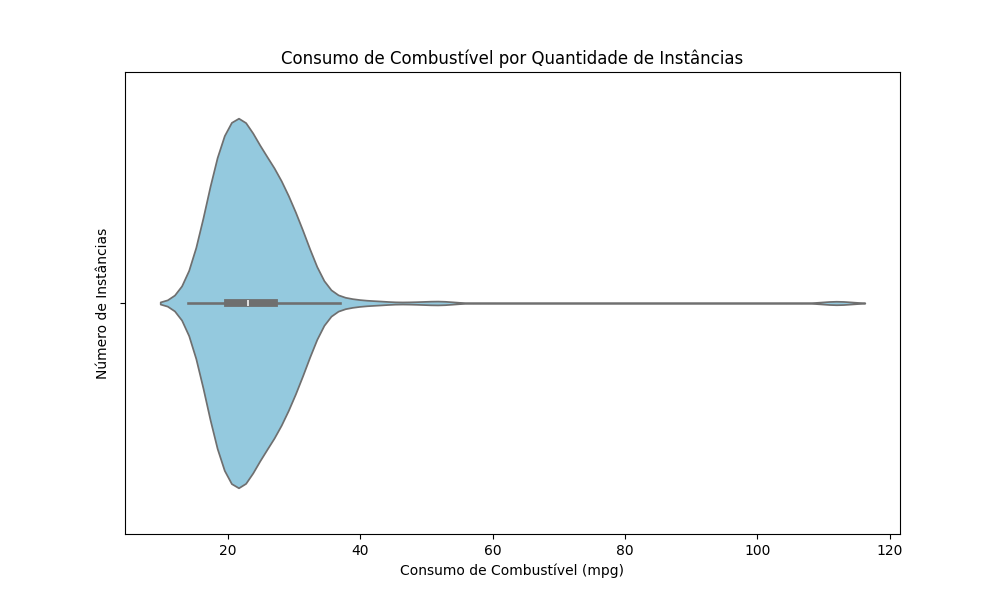
\includegraphics[width=.85\linewidth]{images/plots/violin_plots/pure_combination_mpg.png}
  \caption{\label{img:combination_dist} \textit{Violin Plot} de Consumo Médio}
\end{figure}

Nesse ponto, já se observa que há instâncias problemáticas, claramente \textit{outliers} que devem ser removidas do conjunto de dados. Ademais, a maior concentração dos veículos
apresenta consumo médio entre 15 e 30mpg, algo que pode guiar bastante os modelos. Após isso, analisou-se o atributo de classes de veículos para ter uma ideia da sua distribuição
em um gráfico de setores.

\begin{figure}[h!]
  \centering
  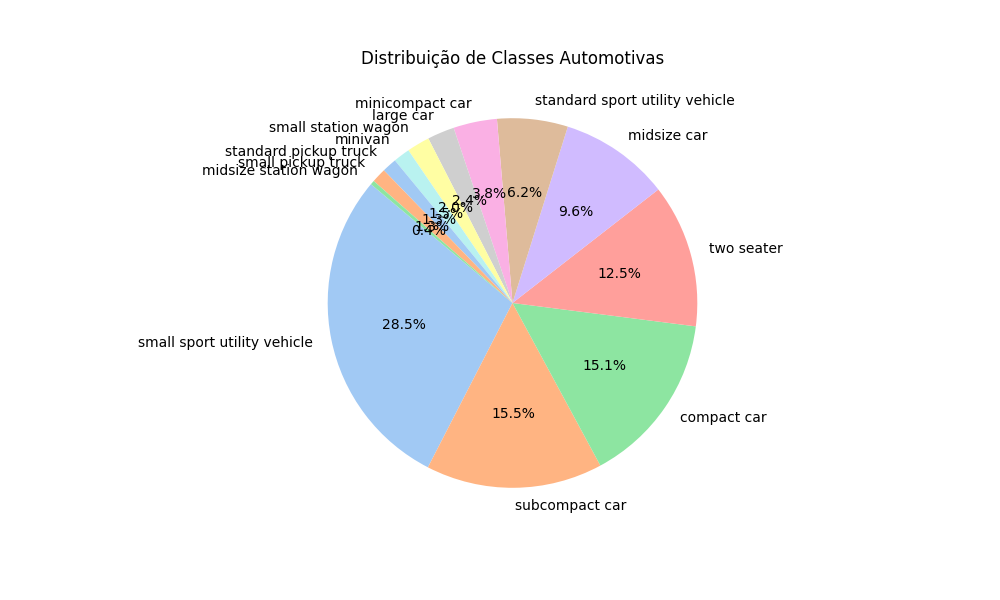
\includegraphics[width=.85\linewidth]{images/plots/pie_charts/pure_car_classes.png}
  \caption{\label{img:classes_dist} Distribuição de Classes de Veículos}
\end{figure}

Com ele, é perceptível que talvez seja necessário agrupar as classes de veículos e outros atributos que contenham classes com muito poucos representantes, como \textit{midsize station wagon},
por exemplo, em uma classe geral chamada \textit{others}. Porém, isso será melhor analisado, se necessário, na segunda etapa do trabalho. No entanto, algo que é necessário é a codificação dos
atributos categóricos em numéricos para padronizar a entrada numérica dos modelos.

Por fim, analisou-se a Correlação de Pearson entre os atributos numéricos através do \textit{heatmap} abaixo:

\begin{figure}[h!]
  \centering
  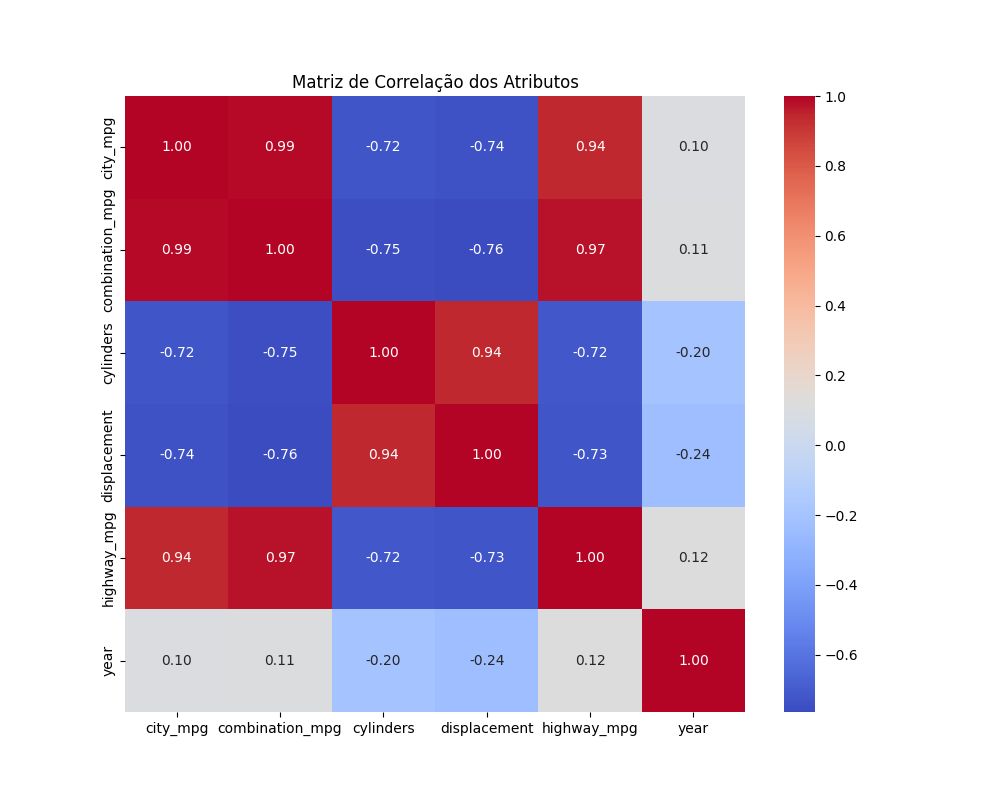
\includegraphics[width=.85\linewidth]{images/plots/heatmaps/numeric_atributes_correlation.png}
  \caption{\label{img:num_heatmat} \textit{Heatmap} de Correlações entre Atributos Numéricos}
\end{figure}

Olhando para o gráfico acima, percebe-se que há diversos atributos preditores que apresentam alto nível de correlação com a saída \textit{combination mpg} e entre si. Ambos os atributos
\textit{highway mpg} e \textit{city mpg} serão descartados do \textit{dataset} por terem alta correlação entre si e com o valor da saída do modelo, facilitando demais a tarefa dos modelos.
Além disso, \textit{displacement} ou (exclusivo) \textit{cylinders} será excluído do conjunto de dados por terem alta correlação entre si.

Isto não foi ilustrado pelos gráficos, porém os dados numéricos apresentam diversas escalas diferentes, exigindo técnicas de normalização após a separação de conjuntos de treinamento/validação
e de testes.

\subsection{Pré-processamento dos Dados}

Como já discutido na seção acima e analisando alguns trabalhos realizados com esse conjunto de dados, esses sendo de Lunovian \cite{Lunovian}, da Ayşe \cite{Ayşe} e do Priyanshu \cite{Priyanshu},
implementou-se algumas estratégias de pré-processamento nos dados deste problema.

Primeiramente, realizou-se a remoção dos atributos discutidos anteriormentes. Esses sendo o \textit{highway mpg}, \textit{city mpg} e \textit{displacement}, visto que apresentam alto níveis de
correlação entre si e com o valor da saída do modelo. Após essa remoção, filtrou-se as instâncias com muitos atributos faltantes (em geral, carros elétricos que funcionam diferentemente dos carros
que funcionam com combustíveis fósseis).

Depois disso, foi realizada a limpeza de instâncias cujo atributo alvo representava um \textit{outlier} no gráfico de distribuição de consumo médio dos veículos. Essa estratégia é necessária para
evitar que os modelos sejam treinados com instâncias que não representam bem a grande a maioria dos veículos. Utilizou-se a medida padrão de 1.5 vezes o IQR para identificar \textit{outliers}.

Sobre a codificação dos atributos, o grupo utilizou a codificação padrão de categórico para numérico que é o \textit{one-hot encoding}. A justificativa para isso é que os atributos categóricos não
apresentam nenhuma ordem específica que justifique utilizar uma codificação em números inteiros. Além disso, em relação à normalização, baseado no trabalho do Jason Brownlee \cite{ColumnTransformer} e
do Matheus Vasconcelos \cite{PadronizarDados}, optou-se por utilizar a padronização por \textit{z-score}, visto que os dados aproximam uma distribuição normal. Tanto a codificação, quanto a normalização
foram aplicadas após a separação de conjuntos de treinamento/validação e de testes.

Um outro problema encontrado consiste na possibilidade de não ser visto algum modelo de carro (\textit{model}) no treinamento. Isso pode acontecer pois há uma quantidade muito grande de modelos diferentes,
alguns deles com poucas instâncias. Para solucionar esse problema, ``forçou-se" a haver pelo menos uma instância de cada modelo de veículo no conjunto de treinamento, antes de realizar a separação de
conjunto de dados para teste. Para realizar essa última separação, utilizou-se a função \texttt{train\_test\_split()} com um \texttt{test\_size} de 15\%.

\section{Abordagem, Algoritmos e Estratégias de Avaliação}

\section{\textit{Spot-checking} de Algoritmos}

\clearpage
\printbibliography
\thispagestyle{empty}

\end{document}